\documentclass[11pt]{article}
\usepackage{graphicx, fancyhdr}
\usepackage{amsmath, amsfonts}
\usepackage{color, hyperref}
\usepackage{enumerate}

\newcommand{\blue}[1]{{\color{blue} #1}}

\setlength{\topmargin}{-.375 in} 
\setlength{\textheight}{8.75 in}
\setlength{\textwidth}{6.5 in} 
\setlength{\evensidemargin}{0 in}
\setlength{\oddsidemargin}{0 in} 
\setlength{\parindent}{0 in}
\newcommand{\ben}{\begin{enumerate}}
\newcommand{\een}{\end{enumerate}}
\newcommand{\dsum} {\displaystyle\sum}

\lhead{Stat 105} 
\chead{Homework Assignment 3} 
\rhead{Due Thursday, February 11} 
\lfoot{Spring 2016} 
\cfoot{\thepage} 
\rfoot{} 
\renewcommand{\headrulewidth}{0.4pt} 
\renewcommand{\footrulewidth}{0.4pt} 

\def\Exp#1#2{\ensuremath{#1\times 10^{#2}}}
\def\Case#1#2#3#4{\left\{ \begin{tabular}{cc} #1 & #2 \phantom
{\Big|} \\ #3 & #4 \phantom{\Big|} \end{tabular} \right.}

\begin{document}
\pagestyle{fancy} 

Show \textbf{all} of your work on this assignment and answer each 
question fully in the given context.

\ben[1.]

\item \textbf{Fire Damage.}

\een

A fire safety inspector wants to relate the amount of fire damage in major residential fires (in thousands of dollars) to distance between the residence and the nearest fire station (in miles). The study was conducted in the suburb of a major city; a sample of 15 recent fires in this suburb is selected. Below is a scatterplot displaying these 15 fires.

\begin{center}
	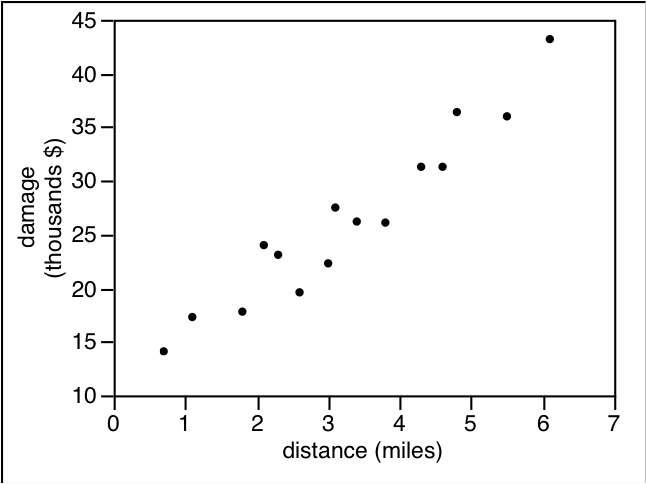
\includegraphics[scale=0.5]{scatter.png}
\end{center}

The following summaries were are computed from the data:
\[
\displaystyle{\sum_{i=1}^{15}} x_i = 49.2 \qquad 
\displaystyle{\sum_{i=1}^{15}} x_i^2 = 196.16 \qquad 
\displaystyle{\sum_{i=1}^{15}} y_i = 396.2 \qquad 
\displaystyle{\sum_{i=1}^{15}} y_i^2 = 11376.48 \qquad 
\displaystyle{\sum_{i=1}^{15}} x_i y_i = 1470.65
\]
It is worth mentioning that $b_1$ can be written in the following ways:

\[
   b_1 = 
   \frac{\sum_{i=1}^n (x_i - \bar{x})(y_i - \bar{y})}{\sum_{i=1}^n (x_i - \bar{x})^2}  = \frac{\sum_{i=1}^n x_i \cdot y_i - n \bar{x} \bar{y}}{\sum_{i=1}^n x_i^2 - n \bar{x}^2}
\]

Use this information to answer the following questions by hand. 
Show all your work and the relevant formulas.

\ben[(a)]
\item Identify the explanatory and response variables for this problem.

\item Does it appear that a linear relationship is appropriate to describe the relationship between fire damage and distance from the fire station? 
If so, is the relationship positive or negative?

\item Calculate the fitted least squares regression equation.

\item Provide an interpretation of the estimated slope \textbf{within the context of the problem.}

\item 
Provide an interpretation of the estimated intercept \textbf{within the context of the problem.} 
Does the estimated value of the intercept make sense? Explain briefly.

\item \label{est} 
Use the fitted least squares regression equation to predict 
the amount of fire damage for a house located 5.5 miles from the nearest
fire station.

\item The actual fire damage for the house in part (f) was 36 thousand 
dollars. Calculate the residual.

\item \label{extrap}
   Use the fitted least squares regression equation to predict the 
amount of fire damage for a house located 30 miles from the nearest
fire station. 

\item Why should we not trust the prediction obtained in part (h)?

\item Give the value of $R^2$ and provide an interpretation of this value within the context of the problem.

\een

\ben[2.]

\item Using \verb!JMP! answer from the text Chapter 4, Section 1, Problem 4 (page 140).
I have already put the data into a \verb!.jmp! file on the course page (\verb!tools.jmp!).
Print and attach all plots requested. The point break down is as follows:

\ben[(a)]

\item 5 points for the plot, 5 points for $R^2$, and 5 pts for the explanation.

\item 5 points for the plot, 5 points for $R^2$, and 5 pts for the explanation.

\item 5 points for the prediction of tool life, 5 points for the discussion of the relationship between x and y. Note that the this means you need to write an equation that relates $x$ and $y$ directly, not $\log(x)$ to $\log(y)$ or $x$ to $\frac{1}{y}$ - an equation using $x$ and $y$. The "\textit{By the way}" part from the book might be helpful here in thinking about the form of the equation.

\een

\een

\end{document}
